% !TEX encoding = UTF-8 Unicode

\documentclass[a4paper]{article}

\usepackage{color}
\usepackage{url}
\usepackage[T2A]{fontenc} % enable Cyrillic fonts
\usepackage[utf8]{inputenc} % make weird characters work
\usepackage{graphicx}
\usepackage{subfig}

\usepackage[english,serbian]{babel}
%\usepackage[english,serbianc]{babel} %ukljuciti babel sa ovim opcijama, umesto gornjim, ukoliko se koristi cirilica

\usepackage[unicode]{hyperref}
\hypersetup{colorlinks,citecolor=green,filecolor=green,linkcolor=blue,urlcolor=blue}

%\newtheorem{primer}{Пример}[section] %ćirilični primer
\newtheorem{primer}{Primer}[section]

\begin{document}

\title{Eliminacija pozadine u video zapisima\\ \small{Seminarski rad u okviru kursa\\Naučno izračunavanje\\ Matematički fakultet}}

\author{\href{mailto:mi14097@matf.bg.ac.rs}{Vesna Katanić}, \href{mailto:mi14022@matf.bg.ac.rs}{Anja Ivanišević}}
\date{14.~septembar 2019.}
\maketitle

\tableofcontents

\newpage

\section{Uvod}
\label{sec:uvod}

Algoritmi za eliminaciju pozadine u video zapisima su algoritmi koji imaju za cilj detekciju kretanja i odvajanje pozadine od objekata koji se kreću. CIlj ovog rada je upoznavanje različitim algoritmima za detekciju kretanja i njihovo poređenje.

\section{Primenjeni algoritmi}
\label{sec:algoritmi}

U ovom radu smo poredili tri različita algoritma za eliminaciju pozadine u video zapisima. Ti algoritmi su: \emph{Basic Motion Detection (BMD)}, \emph{Gaussian Mixture Model (GMM)} i \emph{K Nearest Neighbours (KNN)}. Ideja svakog od ovih algoritama je da transformišu ulazni video u novi video u kojem će pozadina biti ofarbana u crno a objekti koji se kreću u belo, kako bi se oni izdvojili. U nastavku rada će ovi algoritmi biti predstavljeni.

\subsection{Basic Motion Detection}

\emph{Basic Motion Detection} je najjednostavniji algoritam od predstavljenih algoritama. U ovom algoritmu se polazi od pretpostavke da se video $I$ sastoji od statičke pozadine $B$ ispred koje se nalaze objekti koji se kreću. Kako bismo detektovali objekte računa se rastojanje trenutnog modela pozadine i posmatranog frejma. Na osnovu ovog rastojanja pravi se rezultujuća crno-bela slika. 

Model pozadine se ažurira na osnovu prethodnog stanja i trenutno posmatranog frejma po sledećoj formuli: 
$B_{s,t+1} = (1 - \alpha) * B_{s,t} + \alpha * I_{s,t}$
gde je $s$ posmatrani piksel, $t$ posmatrani frejm i $\alpha$ parametar za koju je uzeta vrednost $0.001$. Za početnu vrednost modela pozadine $B$ je uzet prvi frejm, dok je rastojanje između frejma i modela računato na osnovu Euklidskog rastojanja.

\subsection{Gaussian Mixture Model}

Ideja algoritma \emph{Gaussian Mixture Model} jeste da u svakom trenutku $t$ sa osnovu poslednjih $T$ frejmova računamo verovatnoću da se određena boja javi u posmatranom pikselu. Verovatnoća se računa kombinovanjem najviše $M$ Gausovih raspodela po formuli: $p = \sum_{m = 1}^{M} \pi_m N (x, \mu_m, \sigma_m^2)$ , a u kojima konfigurišu parametri $\pi$, $\mu$ i $\sigma^2$ koje iterativno ažuriramo po sledećim formulama: \\
$\pi_m \leftarrow \pi_m + \alpha (\o_m - \pi_m)$,\\
$\mu_m \leftarrow \mu_m + \o_m (\alpha / \pi_m) \delta_m$,\\
$\sigma_m^2 \leftarrow \sigma_m^2 + \o_m (\alpha / \pi_m) (\delta_m^T \delta_m - \sigma_m^2)$.\\
Za svaki novi piksel, parametar $o_m$ će biti jednak $1$ za komponentu sa najvećim $\pi$ ako je \emph{"blizu"} posmatranog piksela, u suprotnom će biti jednak $0$. Kažemo da je piksel \emph{"blizu"} komponente ako je Mahalanobisovo rastojanje manje od neke unapred zadate granice (na primer $3$). Ako nijedna komponenta nije \emph{"blizu"} posmatranog piksela, generišemo novu komponentu sa sledećim parametrima: 

Ako smo dostigli maksimalan broj komponenti $M$, tada ćemo zameniti komponentu sa najmanjom vrednošću parametra $\pi$ sa novokreiranom komponentom.

Model pozadine će se sastojati od $B$ komponenti sa najvećim vrednostima parametra $\pi$, dok će ostale komponente predstavljati objekte koji se kreću. Broj $B$ se računa po formuli:\\
$B = \arg\min_{b} (\sum_{m = 1}^{b} \pi_m > (1 - c_f))$.

Implementacija ovog algoritma postoji u OpenCV biblioteci i nju smo koristili za potrebe ovog rada.

\subsection{K Nearest Neighbours}

Ovaj algoritam predstavlja unapređenje algoritma \emph{Kernel density estimation} algoritma. Za razliku od njega gde smo koristili fiksnu veličinu kernela $D$ ovom algoritmu prilagođavamo $D$ za svaki piksel posebno. Umesto da pokušavamo da nađemo $D$ koje je globalno optimalno, mi povećavamo širinu $D$ dokle god unapred zadata količina podataka nije pokrivena. Na ovaj način dobijamo velike kernele u oblastima sa malom količinom podataka i male kernele gde je gustina podataka veća. Ovaj alogirtam daje jako dobre rezultate ako ima malo objekata koji se kreću. Implementacija ovog algoritma postoji u OpenCV biblioteci i nju smo koristili za potrebe ovog rada.

\section{Evaluacija algoritma}
\label{sec:efikasnost}

Na narednim slikama su redom prikazani ulazna slika i rezultati algoritama \emph{BMD}, \emph{GMM} i \emph{KNN}.


\begin{figure}
    \centering
    \subfloat[Original]{{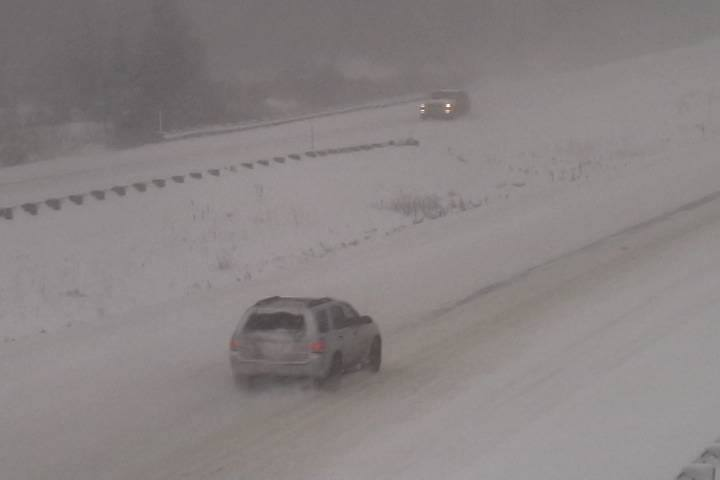
\includegraphics[width=5cm]{dataset/slike/original.jpg} }}
    \qquad
    \subfloat[BMD]{{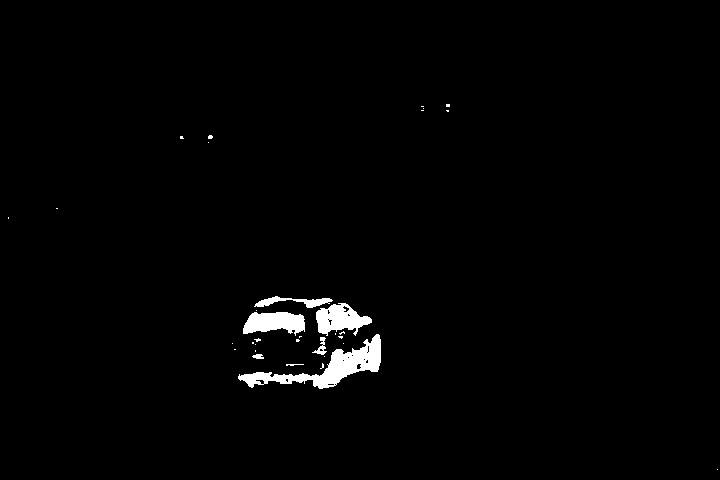
\includegraphics[width=5cm]{dataset/slike/bmd.jpg} }}
    \caption{Originalna slika i rezultat BMD algoritma}}
    \label{fig:example}
\end{figure}

\begin{figure}
    \centering
    \subfloat[GMM]{{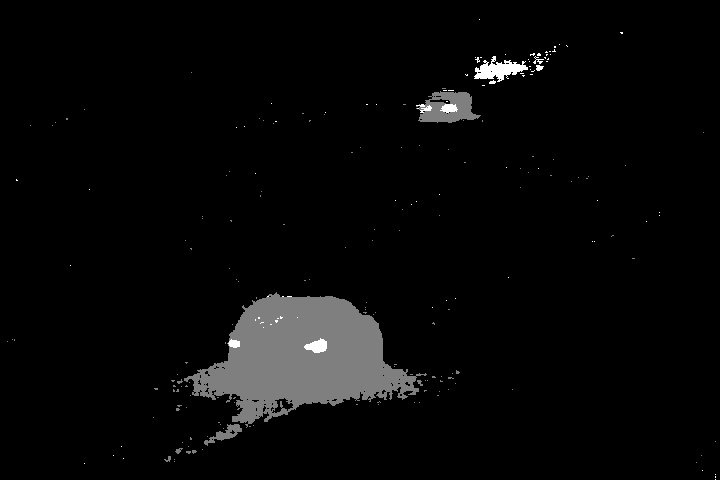
\includegraphics[width=5cm]{dataset/slike/mog2.jpg} }}
    \qquad
    \subfloat[KNN]{{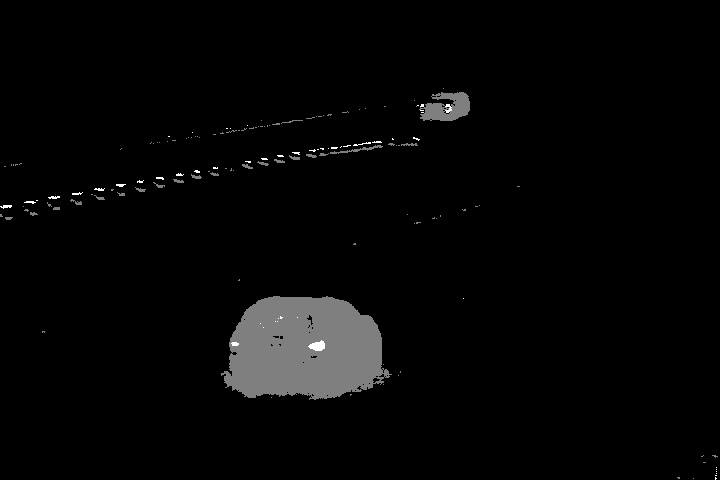
\includegraphics[width=5cm]{dataset/slike/knn.jpg} }}
    \caption{Rezultati GMM i KNN algoritama}}
    \label{fig:example}
\end{figure}

Algoritmi su pokretani na tri vrste test primera - saobraćaj za vreme mećave, saobraćaj u standardnim uslovima i noćni snimak nadzorne kamere. Svaki od algoritama je posmatran kao problem klasifikacije i za evaluaciju rezultata korišćene su mere \emph{Precision}, \emph{Recall} i \emph{F1 mera}.

Ostvareni su sledeći rezulati:

\vspace{5mm}

\begin{tabular}{cc}
    \begin{minipage}{.5\linewidth}
        \begin{tabular}{|l|l|l|}
    \hline
\thead{BMD} & \thead{GMM} & \thead{KNN} \\ 
                    \hline
0.9409 & 0.4237 & 0.5218 \\    \hline
0.4757 & 0.1820 & 0.2738 \\    \hline
0.9822 & 0.8972 & 0.8872 \\    \hline
\end{tabular}
    \end{minipage} &

    \begin{minipage}{.5\linewidth}
        \begin{tabular}{|l|l|l|}
    \hline
\thead{BMD} & \thead{GMM} & \thead{KNN} \\ 
                    \hline
0.4528 & 0.9414 & 0.9157 \\    \hline
0.7833 & 0.8926 & 0.9025 \\    \hline
0.9436 & 0.7184 & 0.9068 \\    \hline
\end{tabular}
    \end{minipage} 
\end{tabular}

\vspace{5mm}

\begin{center}

\begin{tabular}{|l|l|l|}
    \hline
\thead{BMD} & \thead{GMM} & \thead{KNN} \\ 
                    \hline
0,6114 & 0,5844 & 0,6648 \\    \hline
0,5919 & 0,3023 & 0,4201 \\    \hline
0,9625 & 0,7979 & 0,8969 \\    \hline
\end{tabular}
\end{center}


\end{document}
